\section{Theory} \label{sec:theory}


\subsection{Single-layer perceptrons}
The principle behind single-layer perceptrons, which is the simplest neural networks, is quite easy to understand. A set of inputs are sent into the network, and a set of outputs is returned. The inputs are multiplied by several weights, and by adjusting those weights a single perceptron can solve every \textit{linear problem} (I come back to this later). A drawing of the single-layer perceptron is found in figure (\ref{fig:single_perceptron}).

\begin{figure} [H]
	\centering
	\label{fig:single_perceptron}
	\begin{tikzpicture}
	\node[functions] (center) {};
	\node[below of=center,font=\scriptsize,text width=4em] {Activation function};
	\draw[thick] (0.5em,0.5em) -- (0,0.5em) -- (0,-0.5em) -- (-0.5em,-0.5em);
	\draw (0em,0.75em) -- (0em,-0.75em);
	\draw (0.75em,0em) -- (-0.75em,0em);
	\node[right of=center] (right) {};
	\path[draw,->] (center) -- (right);
	\node[functions,left=3em of center] (left) {$\sum$};
	\path[draw,->] (left) -- (center);
	\node[weights,left=3em of left] (2) {$o_2$} -- (2) node[input,left of=2] (l2) {$x_2$};
	\path[draw,->] (l2) -- (2);
	\path[draw,->] (2) -- (left);
	\node[below of=2] (dots) {$\vdots$} -- (dots) node[left of=dots] (ldots) {$\vdots$};
	\node[weights,below of=dots] (n) {$o_n$} -- (n) node[input,left of=n] (ln) {$x_n$};
	\path[draw,->] (ln) -- (n);
	\path[draw,->] (n) -- (left);
	\node[weights,above of=2] (1) {$o_1$} -- (1) node[input,left of=1] (l1) {$x_1$};
	\path[draw,->] (l1) -- (1);
	\path[draw,->] (1) -- (left);
	\node[weights,above of=1] (0) {$o_0$} -- (0) node[input,left of=0] (l0) {$1$};
	\path[draw,->] (l0) -- (0);
	\path[draw,->] (0) -- (left);
	\node[below of=ln,font=\scriptsize] {inputs};
	\node[below of=n,font=\scriptsize] {weights};
	\end{tikzpicture}
	\caption{Single perceptron}
\end{figure}
Initially one needs to train the network such that it knows which outputs are correct, and for that one needs to know the outputs that correspond to the inputs. Every time the network is trained, the weights are adjusted such that the error is smaller. 

The very first step is to calculate the initial outputs, where the weights usually are set to small random numbers. Then the error is calculated, and the weights are updated to minimize the error. So far so good.

\subsubsection{Forward phase}\label{sec:ashortwalkthrough}
Let us look at it from a more mathematical perspective, and calculate the netto output. The netto output seen from an output node is simply the sum of all the "arrows" that go to the node, see figure (\ref{fig:single_perceptron}), where each "arrow" is given by the left-hand node multiplied with its respective weight. For example the contribution from input node 2 to output node 1 follows from $X_2\cdot w_{21}$, and the total netto output to $O_1$ is therefore
\begin{equation}
net_1 = \sum_{i=1}^{I} X_i\cdot w_{i1} + b_1\cdot 1.
\end{equation}
Just some notation remarks: $X_i$ is the value of input node $i$ and $w_{ij}$ is the weight which connects input $i$ to output $j$. The parameter $b$ is the bias weight, which we will discuss later. The netto output to a node $j$ is therefore 
\begin{empheq}[box={\mybluebox[5pt]}]{equation}
net_j = \sum_{i=1}^{I} X_i\cdot w_{ij} + b_j\cdot 1.
\label{eq:forward}
\end{empheq}
You might wonder why we talk about the netto output all the time, do we have other outputs? If we look at the network mathematically, what we talk about as the netto output should be our only output. Anyway, to make the algorithm easy to implement, mapping the netto output to a final output is standard practice. You do not need to care too much about this right now, the mapping is done with a sigmoid function and is explained further in section \ref{sec:sigmoid1}. The sigmoid function takes in the netto output and gives the output, 
\begin{equation}
out_j = \text{sigmoid}(net_j).
\end{equation}
Now all the tools for finding the outputs are in place, and we can calculate the error. If the outputs are larger than the targets (which are the exact answers), the weights need to be reduced, and if the error is large the weights need to be adjusted a lot. The weight adjustment can be done in multiple ways, and we will apply the widely used \textbf{stochastic gradient descent}, which might also be the most basic. The principle is easy: each weight is adjusted with respect to itself total error gradient,
\begin{empheq}[box={\mybluebox[5pt]}]{equation}
w_{ij}^+= w_{ij} - \eta\cdot\frac{\partial E_{TOT}}{\partial w_{ij}},
\label{eq:w_update}
\end{empheq}
where $\eta$ is what we call the learning rate. If not everything is clear right now, it is fine. We will discuss the most important concepts before we dive into the maths.

\subsubsection{BIAS}
As mentioned above, we use biases when calculating the outputs. The nodes, with value $B$, are called the bias nodes, and the weights, $b$, are called the bias weights. But why do we need those? 

Imagine we have two inputs with value zero, and one output which should not be zero (this could for instance be a NOR gate). Without the bias, we will not be able to get any other output than zero, and in fact the network would struggle to find the right weights even if the output had been zero. 

The bias value $B$ does not really matter since the network will adjust the bias weights with respect to it, and is usually set to 1 and ignored in the calculations.

\subsubsection{Learning rate}
In principle the weights could be updated without adding any learning rate ($\eta=1$), but this can in practice be problematic. It is easy to imagine that the outputs can be fluctuating around the targets without decreasing the error, which is not ideal, and a learning rate can be added to avoid this. The downside is that with a low learning rate the network needs more training to obtain the correct targets (and it takes more time), so we need to find a balance. 

The problem occurs when we are close to the target only, so one solution could be using dynamic learning rate, which decreases when the number of iterations increase,
\begin{equation}
\eta=\frac{\eta_0}{\sqrt{1+\text{iter}}},
\end{equation}
where $\eta_0$ is the initial learning rate and iter is the current iteration. 

Regardless of whether we use dynamic or static learning rate, an usual value is in the interval $(0,0.25]$, but it is not unusual to see values as low as 0.01 (especially for the static case). 


\subsubsection{Cost function}\label{sec:error_function}
The cost function we will use is inspired by the error function used in \textbf{least squares methods}, and reads
\begin{empheq}[box={\mybluebox[5pt]}]{equation}
E_{TOT} = \frac{1}{2}\sum_j (y_j - t_j)^2
\label{eq:error_function}
\end{empheq}
where we sum over all the outputs. The factor $1/2$ is added just to give a clean derivative, which in fact makes all the expressions neater. It would also be possible to use other error functions, but to find specific expressions for the weight updating formulas, we better focus on the one above. 

\subsection{Activation function}\label{sec:sigmoid1}
Inspired by Boolian algebra, the inputs and outputs initially are set to either 0, 1, or a superposition of them. To ensure that every output is between 0 and 1, we map them all using a cost function. Perhaps the most common function to use is
\begin{empheq}[box={\mybluebox[5pt]}]{equation}
f(x)=\frac{1}{1+\exp(-x)}
\label{eq:sigmoid}
\end{empheq}
which maps between 0 and 1 as required. Another important property is that the derivative of this function has an easy form, which is important. The derivative of this function is
\begin{equation}
f'(x)=f(1-f)
\end{equation}
and the derivation of it is shown carefully in Appendix A. The function is presented in figure (\ref{fig:sigmoid1}).
\begin{figure} [H]
	\centering
	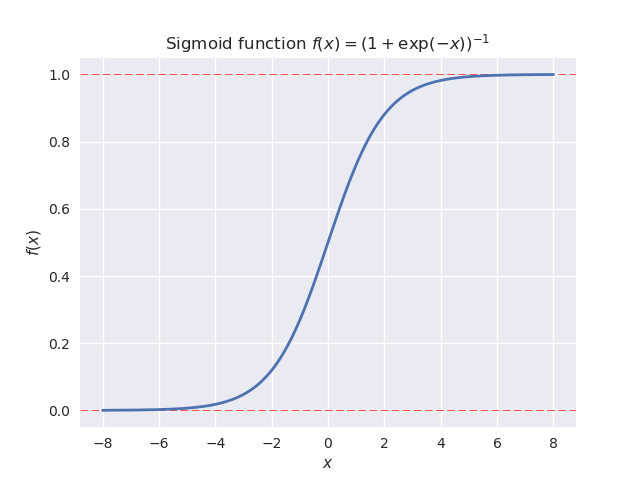
\includegraphics[scale=0.65]{images/sigmoid1.png}
	\caption{A sigmoid function plotted from -8 to 8. The asymphtotes are drawn to stress that the function will approach the value 1 when $x\rightarrow \infty$ and the value 0 when $x\rightarrow -\infty$.}
	\label{fig:sigmoid1}
\end{figure} 

We can also use other sigmoid functions which not even map between 0 and 1, for instance another well-known sigmoid function reads
\begin{empheq}[box={\mybluebox[5pt]}]{equation}
f(x)=\tanh(x)=\frac{\exp(x)-\exp(-x)}{\exp(x) + \exp(-x)}
\end{empheq}
which maps between -1 and 1. Apart from that, the function looks quite similar to the sigmoid function in equation (\ref{fig:sigmoid1})\\
\begin{figure} [H]
	\centering
	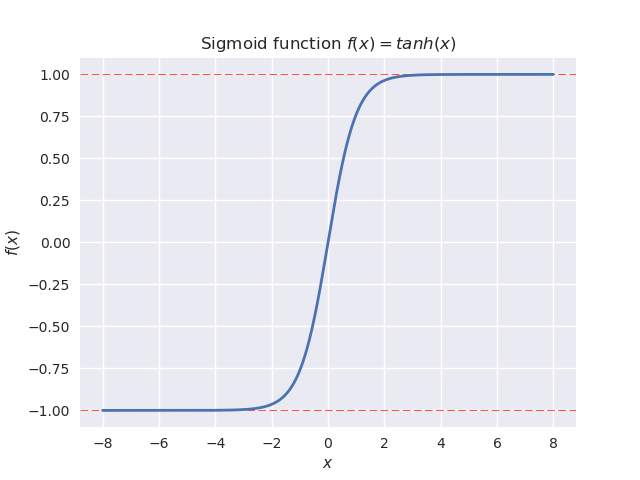
\includegraphics[scale=0.65]{images/sigmoid2.png}
	\caption{A sigmoid function plotted from -8 to 8. The asymphtotes are drawn to stress that the function will approach the value 1 when $x\rightarrow \infty$ and the value -1 when $x\rightarrow -\infty$.}
	\label{fig:sigmoid2}
\end{figure} 
Also this function got a simple derivative, given by
\begin{equation}
\frac{d\tanh(x)}{dx}=\frac{1}{\cosh^2(x)}=\frac{4}{(\exp(x)+\exp(-x))^2}
\end{equation}
which is shown in Appendix B. 

\subsection{Backward phase}
Now we have the fundamentals to go further with the theory expressed in section \ref{sec:ashortwalkthrough}. Actually, the only thing we are left with is finding an expression for the weight updating based on the formula from equation (\ref{eq:w_update}), 
\begin{equation}
w_{ij}^+= w_{ij} - \eta\cdot\frac{\partial E_{TOT}}{\partial w_{ij}},
\end{equation}
where the partial derivative is what we need to find. Since the energy is not directly dependent on $w_{ij}$, we need to do a change of variables such that we get derivatives we can calculate. Probably the best choice is
\begin{equation}
\frac{\partial E_{TOT}}{\partial w_{ij}}=\frac{\partial E_{TOT}}{\partial out_{j}}\cdot\frac{\partial out_{j}}{\partial net_{j}}\cdot\frac{\partial net_{j}}{\partial w_{ij}}.
\end{equation}
Standard differentiating of the error function from section \ref{sec:error_function} gives
\begin{equation}
\frac{\partial E_{TOT}}{\partial out_{j}}=-(t_j-out_j)
\end{equation}
which is a neat expression as pointed out above. To obtain the second fraction, we need to decide which sigmoid function to use. In the calculations I will use the first mentioned in section \ref{sec:sigmoid1}, that reads
\begin{equation}
out_j=\frac{1}{1+\exp(-net_j)}.
\end{equation}
and we have already found that
\begin{equation}
\frac{\partial out_{j}}{\partial net_{j}}=out_j(1-out_j).
\end{equation}
Furthermore the netto output is given by equation (\ref{eq:forward}),
\begin{equation}
net_j = \sum_{i=1}^{I} X_i\cdot w_{ij} + b_j\cdot 1,
\end{equation}
which simply gives
\begin{equation}
\frac{\partial net_{j}}{\partial w_{ij}}=X_i.
\end{equation}
We end up with 
\begin{equation}
\frac{\partial E_{TOT}}{\partial w_{ij}}=-(t_j-out_j)\cdot out_j(1-out_j)\cdot X_i
\end{equation}
and the weight updating formula
\begin{empheq}[box={\mybluebox[5pt]}]{equation}
w_{ij}^{+}=w_{ij} + \eta\cdot(t_j-out_j)\cdot out_j(1-out_j)\cdot X_i
\end{empheq}
Similarly we need to update the bias weights, with a formula similar to that one in equation (\ref{eq:w_update}):
\begin{equation}
b_i^+=b_i - \eta\cdot\frac{\partial E_{TOT}}{\partial b_i}.
\end{equation}
We do the same change of variables and the only thing that changes is the last part, $\partial net_i/\partial b_i$, which can easily be found to be 1. Then
\begin{empheq}[box={\mybluebox[5pt]}]{equation}
b_i^+=b_i + \eta\cdot(t_i-out_i)\cdot out_i(1-out_i)
\end{empheq}
and all the basics for the single perceptron are set. 